\documentclass[pdftex,12pt,a4paper]{article}
\usepackage[pdftex]{graphicx}
\usepackage{xcolor}
\usepackage{marginnote}
\usepackage{enumitem}
\usepackage{listings}
\usepackage{color}
\usepackage{url}
\usepackage[bottom=1.5cm, outer=5cm, inner=2cm, heightrounded,
marginparwidth=4cm, marginparsep=0.5cm]{geometry}

\definecolor{mygreen}{rgb}{0,0.6,0}
\definecolor{mygray}{rgb}{0.5,0.5,0.5}
\definecolor{mymauve}{rgb}{0.58,0,0.82}

\lstset{ %
  backgroundcolor=\color{white},   % choose the background color; you must add \usepackage{color} or \usepackage{xcolor}
  basicstyle=\footnotesize,        % the size of the fonts that are used for the code
  breakatwhitespace=false,         % sets if automatic breaks should only happen at whitespace
  breaklines=true,                 % sets automatic line breaking
  captionpos=b,                    % sets the caption-position to bottom
  commentstyle=\color{mygreen},    % comment style
  deletekeywords={...},            % if you want to delete keywords from the given language
  escapeinside={\%*}{*)},          % if you want to add LaTeX within your code
  extendedchars=true,              % lets you use non-ASCII characters; for 8-bits encodings only, does not work with UTF-8
  frame=single,                    % adds a frame around the code
  keepspaces=true,                 % keeps spaces in text, useful for keeping indentation of code (possibly needs columns=flexible)
  keywordstyle=\color{blue},       % keyword style
  morekeywords={*,...},            % if you want to add more keywords to the set
  numbers=left,                    % where to put the line-numbers; possible values are (none, left, right)
  numbersep=5pt,                   % how far the line-numbers are from the code
  numberstyle=\tiny\color{mygray}, % the style that is used for the line-numbers
  rulecolor=\color{black},         % if not set, the frame-color may be changed on line-breaks within not-black text (e.g. comments (green here))
  showspaces=false,                % show spaces everywhere adding particular underscores; it overrides 'showstringspaces'
  showstringspaces=false,          % underline spaces within strings only
  showtabs=false,                  % show tabs within strings adding particular underscores
  stepnumber=1,                    % the step between two line-numbers. If it's 1, each line will be numbered
  stringstyle=\color{mymauve},     % string literal style
  tabsize=2,                       % sets default tabsize to 2 spaces
}

\begin{document}
    % Custom title page
    \begin{titlepage}
        \begin{center}
            
\includegraphics[width=5cm]{figures/kulogo}\\[1cm]
            {\Large \bfseries
                Spring 2015\\
                Computer Networks\\
                CMPE324\\[1cm]
            }
            {\large \bfseries
                \noindent Laboratory Experiment No. 7: Introduction to the Application Layer\\[1cm]
            }
        \end{center}

        \noindent \textbf{Aims and Objectives:}
            \begin{itemize}[leftmargin=4cm]
                \item Introduce students to the application layer and socket
                programming.
            \end{itemize}
            \vspace{0.5cm}

        \noindent \textbf{Materials Required:}
            \begin{itemize}[leftmargin=4cm]
                \item IP routers,
                \item Ethernet switches,
                \item PCs with Ethernet adapters,
                \item and straight-through/crossover/rollover cables.
            \end{itemize}
            \vspace{0.5cm}

        \noindent \textbf{Change Log:}
            \begin{itemize}[leftmargin=4cm]
                \item 26-3-2015: original document -- mkhonji.
            \end{itemize}
    \end{titlepage}
    \newpage

    % Lab script content
    \section{Introduction}
        In this introduction, the basic functionality of the HTTP protocol is
        introduced, followed by an introduction to socket programming.

        \subsection{Hypertext Transfer Protocol (HTTP)}
            HTTP is an application-layer protocol. Therefore, it resides in the
            \emph{payload} section of layer 4 protocols (such as TCP and UDP).

            HTTP is a fairly extensive protocol. However, the basic
            functionality of HTTP is fairly simple. In this lab we cover simple
            GET requests and responses.

            A HTTP GET request is presented in Figure \ref{fig:getreq}. Note
            the following:
            \begin{itemize}
                \item This is a minimalist HTTP request. A normal HTTP request
                has more content (as you will observe in later sections).
                \item This HTTP request has a single header field that is the
                \emph{request-line}.
                \item The request-line has a request of type GET. Note that
                    other request types exist, however for simplicity we shall
                    only cover GET requests.
                \item Note that the request line is terminated by CRLF
                    (carriage-return followed by line-feed).
                \item Note that the request header is terminated by another.
                    CRLF.
            \end{itemize}
            \begin{figure}[tbh]
                \centering
                \lstinputlisting[language=HTML]{./html/request}
                \caption{A minimalist GET request.}
                \label{fig:getreq}
            \end{figure}

            An example of a minimalist HTTP response to the request above can
            be as presented in Figure \ref{fig:response}. Note the following:
            \begin{itemize}
                \item This is a minimalist response. Usually, a HTTP response
                    contains more data (as you will observe in later sections).
                \item The first line in the response is the \emph{status-line}
                    that is terminated by CRLF. This line indicates the
                    \emph{status code}, which is 200 in this example. As per
                    the standard, 200 indicates that the request was
                    successfully. This line also contains a \emph{status
                    phrase}, which is ``\emph{OK}'' in this case. Such phrases
                    were useful when web clients were interactive, however
                    modern GUI HTTP clients should ignore such phrases as per
                    the RFC7230.
            \end{itemize}
            \begin{figure}[tbh]
                \centering
                \lstinputlisting[language=HTML]{./html/response}
                \caption{A minimalist HTTP response.}
                \label{fig:response}
            \end{figure}

            This lab describes the most commonly used version of HTTP to date,
            which is version 1.1. Further details on this can be found in
            RFC7230, RFC7231, RFC7233, RFC7234, RFC7235. However, note that
            recently (relative to the time this lab script is written), 17th of
            Feb 2015, IESG has approved HTTP version 2 as a Proposed Standard.

        \subsection{Socket Programming}
            In the previous labs, you were bypassing most forms of automation
            (except those imposed upon us by the hardware). This allowed us to
            craft Ethernet frames, IP packets, and TCP/UDP messages manually
            for experimental purposes.

            However, the problem with such approach is that it's tedious, error
            prune and inefficient. One cannot efficiently implement the whole
            TCP/IP stack every time a new application is coded specially that
            such networking stacks are fairly broad. This can lead into code
            bloat, increased probability of errors/bugs as well as wasted
            developer time.

            In this lab, we will develop applications that use TCP, IP and
            Ethernet without manually implementing the protocols as we did in
            previous labs. Thanks to \emph{socket programming}, this can be
            achieved, transparently, by a few function calls.

            This lab is limited to TCP. However, such concepts can be easily
            extended to UDP as well.

            For your reference, skim throughout the manual pages \emph{tcp(7)}
            and \emph{udp(7)}. When using a POSIX-compliant operating system
            (such as most Linux distributions), such manual pages can be viewed
            by commands \texttt{man 7 tcp} and \texttt{man 7 udp} respectively.

            \textbf{Note:} as the HTTP protocol follows a \emph{client-server}
            model, we will be using terms \emph{client} and \emph{server} to
            describe TCP peers. However, note that TCP ---itself--- is fairly
            general and does not \emph{necessarily} require following a
            client-server model. For example, BitTorrents is an example
            peer-to-peer model that uses TCP.

            \subsubsection{TCP Server}
                \begin{enumerate}
                    \item Obtain a TCP socket as presented in Figure
                        \ref{fig:socket}. \texttt{AF\_INET} refers to IPv4,
                        \texttt{SOCK\_STREAM} refers to reliable bi-directional
                        sequenced sockets. 0 is essentially the protocol number. Since
                        usually only TCP is the only available protocol for
                        \texttt{SOCK\_STREAM}, the protocol number is set to 0.
                        Note that, in order to use the \texttt{socket}
                        function, you have to include the listed header files.
                        \begin{figure}[tbh]
                            \centering
                            \lstinputlisting[language=C]{./html/tcpsocket}
                            \caption{The synopsis of the \texttt{socket} function.}
                            \label{fig:socket}
                        \end{figure}
                    \item Bind that socket to a local address and port using
                        the function \texttt{bind} as presented in Figure
                        \ref{fig:bind}. \texttt{socfd} is the socket obtained
                        in the earlier step.  \texttt{addr} is a pointer to a
                        structure that contains information with regards to the
                        local address and port number to listen to.
                        \texttt{addrlen} specifies the size of the structure
                        \texttt{addr} in bytes.
                        \begin{figure}[tbh]
                            \centering
                            \lstinputlisting[language=C]{./html/tcpbind}
                            \caption{The synopsis of the \texttt{bind} function.}
                            \label{fig:bind}
                        \end{figure}
                    \item Now that the socket is binded to a local address and
                        port, start listening on it by calling the function
                        \texttt{listen} as presented in Figure
                        \ref{fig:listen}.  \texttt{sockfd} is the socket binded
                        earlier.  \texttt{backlog} is the maximum number number
                        of connections that are waiting to be accepted. Your
                        application must ensure that the backlog queue is never
                        full or new connections will get refused. At this stage
                        \texttt{netstat -lp} shall show that your application
                        is listening on the set address and port numbers.
                        \begin{figure}[tbh]
                            \centering
                            \lstinputlisting[language=C]{./html/tcplisten}
                            \caption{The synopsis of the \texttt{listen} function.}
                            \label{fig:listen}
                        \end{figure}
                    \item Accept incoming connections from TCP clients
                        by calling the function \texttt{accept} as presented in
                        Figure \ref{fig:accept}. By default, this function
                        shall \emph{block} for until a connection from a client
                        is established after which it returns a
                        \emph{connection socket} between the local server and
                        the remotely connected TCP client. \texttt{addr2} is a
                        memory structure that will get populated by the address
                        of the connected peer in case your application needs
                        this information, and \texttt{addrlen2} is the length
                        of this memory structure. When your application does
                        not need to analyze the client connection information,
                        you may replace \texttt{addr2} by \texttt{NULL} and
                        \texttt{addrlen2} by \texttt{NULL} as well.
                        \begin{figure}[tbh]
                            \centering
                            \lstinputlisting[language=C]{./html/tcpaccept}
                            \caption{The synopsis of the \texttt{accept} function.}
                            \label{fig:accept}
                        \end{figure}
                    \item Finally, once a connection socket
                        \texttt{conn\_sockfd} is obtained, you can read data
                        from it (octets sent to you by the client) and write
                        data to it (octets sent by you to the client). The
                        networking stack of the kernel will then take care of
                        the remaining networking details (i.e. Ethernet, IP and
                        TCP headers). Quite simply, the read and write
                        operations can be performed by the functions
                        \texttt{read} and \texttt{write} respectively, as
                        presented in Figures \ref{fig:read} and \ref{fig:write}
                        respectively. Alternatively, you can use the functions
                        \texttt{recv} and \texttt{send} when in need of setting
                        additional arguments.
                        \begin{figure}[tbh]
                            \centering
                            \lstinputlisting[language=C]{./html/tcpread}
                            \caption{The synopsis of the \texttt{read} function.}
                            \label{fig:read}
                        \end{figure}
                        \begin{figure}[tbh]
                            \centering
                            \lstinputlisting[language=C]{./html/tcpwrite}
                            \caption{The synopsis of the \texttt{write} function.}
                            \label{fig:write}
                        \end{figure}
                    \item To terminate a connection socket
                        \texttt{conn\_sockfd}, simply use the function
                        \texttt{close} as presented in Figure \ref{fig:close}.
                        At this stage, you can observe the 3-way or 4-way
                        \emph{FIN} handshake.
                        \begin{figure}[tbh]
                            \centering
                            \lstinputlisting[language=C]{./html/tcpclose}
                            \caption{The synopsis of the \texttt{close} function.}
                            \label{fig:close}
                        \end{figure}
                \end{enumerate}

            \subsubsection{TCP Client}
                \begin{enumerate}
                    \item Obtain a socket using the function \texttt{socket}.
                    \item Connect to the remote server using the function
                        \texttt{connect} as presented in Figure
                        \ref{fig:connect}. The TCP connection will be
                        established against the server described in the
                        structure \texttt{addr}. Once the connection is
                        established, this function then returns a
                        connection socket \texttt{conn\_sockfd}.
                        \begin{figure}[tbh]
                            \centering
                            \lstinputlisting[language=C]{./html/tcpconnect}
                            \caption{The synopsis of the \texttt{connect} function.}
                            \label{fig:connect}
                        \end{figure}
                    \item Application layer data can be read and written by using
                        functions \texttt{read} and \texttt{write} respectively
                        as presented in Figures \ref{fig:read} and
                        \ref{fig:write} respectively.
                    \item Finally, when the client finishes reading/writing the
                        data it is supposed to, the connection can be finished
                        by calling \texttt{close} as presented in Figure
                        \ref{fig:close}.
                \end{enumerate}

            \subsubsection{How to Populate \texttt{addr}?}
                 Figure \ref{fig:tcpaddr} presents a code snippet that
                 initializes the \texttt{addr}. The function \texttt{memset} is
                 presented in Figure \ref{fig:memset}. The function
                 \texttt{inet\_addr} essentially takes the dotted-decimal IPv4
                 address from its input string and returns its corresponding
                 unsigned 32bit number.
                 \begin{figure}[tbh]
                     \centering
                     \lstinputlisting[language=C]{./html/tcpaddr}
                     \caption{A code snippet for setting \texttt{addr}.}
                     \label{fig:tcpaddr}
                 \end{figure}
                 \begin{figure}[tbh]
                     \centering
                     \lstinputlisting[language=C]{./html/tcpmemset}
                     \caption{The synopsis of the function \texttt{memset}.}
                     \label{fig:memset}
                 \end{figure}
                 \begin{figure}[tbh]
                     \centering
                     \lstinputlisting[language=C]{./html/tcpinetaddr}
                     \caption{The synopsis of the function \texttt{addr}.}
                     \label{fig:inetaddr}
                 \end{figure}
                

            \subsubsection{Error Codes}
                It's critical to test the returned values of the called
                functions to identify errors early. Below is a high-level list
                of functions and their respective error codes.
                \begin{itemize}
                    \item \texttt{socket} --- returns -1 on error.
                    \item \texttt{bind} --- returns -1 on error.
                    \item \texttt{listen} --- returns -1 on error.
                    \item \texttt{accept} --- returns -1 on error.
                    \item \texttt{read} --- returns -1 on error.
                    \item \texttt{write} --- returns -1 on error.
                    \item \texttt{close} --- returns -1 on error.
                    \item \texttt{connect} --- returns -1 on error.
                \end{itemize}
            


    \section{Lab Preparation}
        \begin{enumerate}
            \item Connect a PC to the routers console port using a rollover
                cable\footnote{If using Linux: \texttt{screen /dev/ttySx} were
                \texttt{x} is the
                serial interfaces ID that is connected to the console
                cable. If using Windows: Use Hyperterminal or Putty to
                connect to \texttt{COMx} ports.}.
            \item Erase the configuration of the
                routers\footnote{\texttt{enable}, \texttt{erase
                startup-config}, \texttt{reload}, and make sure to answer
                \texttt{no} to all yes/no questions while hitting
                \emph{enter} for all \texttt{confirm} prompts.}.
            \item Connect a PC to the switches console ports using rollover
                cables.
            \item Erase the configuration of the
                switch\footnote{\texttt{enable}, \texttt{erase startup-config},
                \texttt{delete vlan.dat}, \texttt{reload}, and answer
                \texttt{no} to all yes/no questions while hitting
                \emph{enter} for all \texttt{confirm} prompts.}.
            \item Run Wireshark on all involved lab PCs as depicted in Figure
                \ref{fig:labtop}.
            \item Physically connect the lab as depicted in Figure \ref{fig:labtop}.
            \item Configure the interfaces:
                \begin{itemize}
                    \item Configure\footnote{\texttt{enable}, \texttt{configure
                        terminal}, \texttt{interface Gi0/0}, \texttt{ip address
                        10.0.0.1 255.255.255.0}.} \texttt{R1}'s interfaces as follows:
                        \begin{itemize}
                            \item GigabitEthernet 0/0: IPv4 address 10.0.12.1,
                                subnet mask 255.255.255.0.
                            \item GigabitEthernet 0/1: IPv4 address 10.0.1.1,
                                subnet mask 255.255.255.0.
                        \end{itemize}
                    \item Configure \texttt{R2}'s interfaces as follows:
                        \begin{itemize}
                            \item GigabitEthernet 0/0: IPv4 address 10.0.12.2,
                                subnet mask 255.255.255.0.
                            \item GigabitEthernet 0/1: IPv4 address 10.0.2.1,
                                subnet mask 255.255.255.0.
                        \end{itemize}
                    \item Configure\footnote{\texttt{ifconfig eth0 10.0.1.2/24}}
                        \texttt{\texttt{PC1}}'s interfaces as follows:
                        \begin{itemize}
                            \item eth0: IPv4 address 10.0.1.2,
                                subnet mask 255.255.255.0.
                        \end{itemize}
                    \item Configure \texttt{\texttt{PC2}}'s interfaces as follows:
                        \begin{itemize}
                            \item eth0: IPv4 address 10.0.2.2,
                                subnet mask 255.255.255.0.
                        \end{itemize}
                \end{itemize}
                
            \item Then add the IP routing tables as follows:
                \begin{itemize}
                    \item For R1: \texttt{ip route 10.0.2.0 255.255.255.0
                        10.0.12.2}
                    \item For R2: \texttt{ip route 10.0.1.0 255.255.255.0
                        10.0.12.1}
                    \item For PC1: \texttt{route add -net 0.0.0.0/0 gw
                        10.0.1.1}
                    \item For PC2: \texttt{route add -net 0.0.0.0/0 gw
                                10.0.2.1}
                \end{itemize}
            \item Test connectivity using the \texttt{ping} command to send
                ICMP Echo messages to PCs in other networks and receive the
                respective ICMP Echo-Reply messages back.
        \end{enumerate}

        \begin{figure}[tbh]
            \centering
            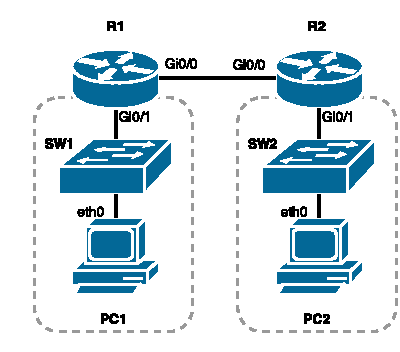
\includegraphics[width=0.6\textwidth]{figures/labtop}
            \caption{Physical lab topology.}
            \label{fig:labtop}
        \end{figure}

    \section{Lab Experiments}
        \subsection{Analyze a Reference HTTP Implementation}
            \begin{flushright}
                \textbf{[40 points]}\marginnote{\small \textbf{Note:} When
                done, present your work to the lab instructor.}
            \end{flushright}

            Throughout the steps below, \emph{PC1} will be the web server that
            by which resources are published via a HTTP web server, and
            \emph{PC2} will be the web client by which resources are requested
            and rendered via a web browser.
            
            \subsubsection{Prepare a Web Server on PC1}
                You are free to install any web server. However, this section
                presents the steps needed to setup Apache HTTPD as it is
                pre-installed in Kali Linux.

                \begin{enumerate}
                    \item Start the web server\footnote{Either by using the
                        command \texttt{service apache2 start}, or the GUI
                        \emph{Applications $\rightarrow$ Kali Linux
                        $\rightarrow$ System Services $\rightarrow$ HTTP
                        $\rightarrow$ apache2 start}}.
                \end{enumerate}

            \subsubsection{Publish Resources Over HTTP}
                Using your preferred text editor, create a few pages in your
                HTTP server's document root\footnote{\texttt{/var/www/}} as
                follows:

                Create files \texttt{/var/www/index.html} and 
                \texttt{/var/www/blog.html} with the contents as presented in
                Figures \ref{fig:index.html} and \ref{fig:blog.html}
                respectively.
                \begin{figure}[tbh]
                    \centering
                    \lstinputlisting[language=HTML]{./html/index.html}
                    \caption{Index's content.}
                    \label{fig:index.html}
                \end{figure}

                \begin{figure}[tbh]
                    \centering
                    \lstinputlisting[language=HTML]{./html/blog.html}
                    \caption{Blog's content.}
                    \label{fig:blog.html}
                \end{figure}

            \subsubsection{Access Your Published Content Over HTTP}
                \begin{enumerate}
                    \item From \emph{PC1} and using a web browser, view your
                    page. In Kali Linux, \texttt{iceweasel} is a pre-installed
                    browser that you may use.

                    \item Analyze transmitted and received datagrams over the
                    network and observe the structure of the HTTP protocol.

                    \item Answer the following questions after analyzing the
                    HTTP requests and responses:
                        \begin{enumerate}
                            \item Identify when the TCP 3-way handshake, data
                                transmission, and connection termination accor,
                                and explain how such events are related to your
                                interaction with the web browser.
                            \item What is the TCP destination port number of
                            the HTTP request?
                            \item Note that you did not specify a destination
                            port number in your web browser. Why did the web
                            browser choose the port number?
                            \item What is the TCP source port number of the
                            HTTP request?
                            \item How do the above port numbers in the HTTP
                            request message (source and destination) relate to
                            those of the HTTP response message?
                            \item What is the request-line of the HTTP request?
                            \item What is the status-line of the HTTP response?
                            \item What is the termination sequence for HTTP
                            header fields?
                            \item What is the separation sequence between HTTP
                            fields and the message body?
                        \end{enumerate}
                \end{enumerate}

        \subsection{Implement a Minimalist Netcat Server}
            \begin{flushright}
                \textbf{[30 points]}\marginnote{\small \textbf{Note:} When
                done, present your work to the lab instructor.}
            \end{flushright}

            Using the procedures described in the introduction section, implement a netcat server that:
            \begin{itemize}
                \item Listens on your local IP address and TCP port 80.
                \item When a \texttt{nc} client connects to it, it should print
                    the data that the client sends to it to its \texttt{STDERR}.
                \item When a client disconnects, the server remains running and
                    able to accept new connections from other \texttt{nc} clients.
            \end{itemize}

        \subsection{Implement a Minimalist HTTP Server}
            \begin{flushright}
                \textbf{[30 points]}\marginnote{\small \textbf{Note:} When
                done, present your work to the lab instructor.}
            \end{flushright}

            Modify your your minimalist netcat server code such that:
            \begin{itemize}
                \item The server parses the request and attempts to identify
                    the requested resource. The server is expected to atleast
                    support the \emph{GET} HTTP requests. 
                \item Based on the requested URL, the server responds by
                    sending the content associated with the requested URL to
                    the requesting client.
                \end{itemize}

            \textbf{Notes:}
            \begin{itemize}
                \item As this is a minimalist experimental web server, you can
                    ignore aspects that relate to the performance of the
                    server.  E.g. it does not have to serve requests
                    \emph{concurrently}.
                \item To simplify your programming, you are allowed to store
                    the content of your resources in strings in your minimalist
                    web server.
                \item Ensure the correct functionality of your HTTP server by
                    accessing the resources \texttt{index.html} and
                    \texttt{blog.html} using your favorite web browser.
            \end{itemize}


\end{document}
